%% ============================================================
%% Forecasting of Energy Prices Using Economic Indicators and
%% GDELT Derived News Signals
%% Springer Nature article -- structure, formatting, and style
%% follow the sn-jnl template; class is portable `article'.
%%
%% PRIMARY (Springer Nature class):
%%   \documentclass[sn-mathphys,Numbered]{sn-jnl}
%% PORTABLE FALLBACK (default below): plain article class so the
%% manuscript compiles on any standard TeXLive install.
%% Compile with: pdflatex main; pdflatex main (figures use PDF
%% versions of the SVG artefacts, generated alongside this file).
%% ============================================================
\documentclass[11pt,a4paper]{article}

%%%% Standard Packages %%%%%%%%%%%%%%%%%%%%%%%%%%%%%%%%%%%%%%%%%%
\usepackage[margin=1in]{geometry}%
\usepackage{graphicx}%
\usepackage{multirow}%
\usepackage{amsmath,amssymb,amsfonts}%
\usepackage{amsthm}%
\usepackage{mathrsfs}%
\usepackage[title]{appendix}%
\usepackage{xcolor}%
\usepackage{textcomp}%
\usepackage{booktabs}%
\usepackage{enumitem}%
\usepackage{listings}%
\usepackage{url}%
\usepackage{authblk}%
\usepackage[numbers,square,sort&compress]{natbib}%
\usepackage{hyperref}%
\usepackage{tikz}%
\usetikzlibrary{arrows.meta,calc,positioning}%
\setlength{\emergencystretch}{3em}
%%%%%%%%%%%%%%%%%%%%%%%%%%%%%%%%%%%%%%%%%%%%%%%%%%%%%%%%%%%%%%%%

% Final paper source. Required figures are stored locally in figures/.
\graphicspath{{figures/}{./}}

% Springer-style helper macros (no-ops in the fallback class).
\newcommand{\bmhead}[1]{\paragraph{\textbf{#1}}}
\newcommand{\backmatter}{}

\raggedbottom

\title{Forecasting of Energy Prices Using Economic Indicators and GDELT Derived News Signals}

\author[1]{Aswin Balaji Thippa Ramesh$^{\ast}$}
\author[1]{Vishal Balaji Fulsundar$^{\dagger}$}
\author[1]{Amir Hossein Jafari$^{\ddagger}$}
\affil[1]{Data Science Program, The George Washington University, Washington, DC, USA}
\date{\small
Corresponding author(s). E-mail(s): \href{mailto:at119@gwu.edu}{at119@gwu.edu};\\
Contributing authors: \href{mailto:vishal.fulsundar@gwu.edu}{vishal.fulsundar@gwu.edu}; \href{mailto:ajafari@gwu.edu}{ajafari@gwu.edu};\\
$^\dagger$These authors contributed equally to this work.\\[0.5em]
April 2026}

\begin{document}
\maketitle

%%==================================================================%%
\begin{abstract}
Energy price forecasting is challenging because crude oil and natural gas prices respond to endogenous price dynamics, macroeconomic conditions, and external narrative signals. This study presents a reproducible evaluation framework for forecasting West Texas Intermediate crude oil and Henry Hub natural gas prices using three information settings: price history alone, macroeconomic indicators from the Federal Reserve Economic Data repository, and news-derived signals from the Global Database of Events, Language, and Tone. The analysis applies a common walk-forward evaluation protocol across daily and monthly frequencies and compares univariate and multivariate forecasting approaches under the same data preparation, split construction, and metric reporting procedures. The objective is not only to estimate future price paths, but also to examine how endogenous and exogenous information sources affect forecast stability across commodities and sampling frequencies. All reported values are traced to stored metric tables, forecast plots, and diagnostic artifacts in the project repository, preserving reproducibility and factual consistency.

\medskip
\noindent\textbf{Keywords:} Energy price forecasting; Crude oil; Natural gas; GDELT; FRED macroeconomic indicators; Exogenous regressors; Time series evaluation.
\end{abstract}

%%==================================================================%%
\section{Introduction}\label{sec:intro}

Crude oil and natural gas occupy a structural position in global production, transportation, and inflation transmission, and their spot prices serve as leading indicators of macroeconomic stress~\citep{kilian2009not, hamilton2009causes, baumeister2016forty}. The two commodities exhibit several stylised features that complicate point forecasting: heavy-tailed return distributions, persistent stochastic volatility, regime-switching behaviour around geopolitical and policy events, and a comparatively low signal-to-noise ratio at the daily horizon. These features motivate two complementary forecasting perspectives. Univariate, or endogenous, approaches use the historical price path itself to capture persistence and seasonal structure. Multivariate, or exogenous, approaches augment the price history with macroeconomic indicators and news-derived variables that may represent external demand, supply, policy, or sentiment conditions.

A complementary stream of research has explored the value of news and sentiment-derived signals for forecasting commodity prices~\citep{tetlock2007giving, shapiro2022measuring, baker2016measuring}. The Global Database of Events, Language, and Tone (GDELT) provides one of the largest publicly available, machine-coded event streams covering global media coverage~\citep{leetaru2013gdelt} and supplies engineered features such as the Goldstein conflict-cooperation score~\citep{goldstein1992conflict}, the average tone of the underlying article cluster, and a categorical event-type code based on the CAMEO ontology. Despite the conceptual appeal of fusing these narrative signals with macroeconomic regressors, an exhaustive, like-for-like evaluation of endogenous and exogenous forecasting approaches under the same data pipeline and forecasting protocol remains limited in the open literature.

This work develops such an evaluation framework. Two energy targets are studied --- WTI crude oil (FRED series \texttt{DCOILWTICO}) and Henry Hub natural gas (FRED series \texttt{DHHNGSP}) --- at both daily and monthly frequencies. The exogenous regressor design is structured into three nested input sets: a macroeconomic block of FRED series, a news block engineered from the GDELT event stream, and the union of the two. The comparison is organised around price-only, macro-only, news-only, and news-plus-macro inputs so that the contribution of each information source can be examined under a consistent evaluation design.

The contributions of this paper are as follows. First, the paper introduces a reproducible experimental matrix in which each completed configuration produces a metric panel and a forecast plot, with every reported number stored as a CSV table or vector graphic in the project repository. Second, it provides a side-by-side comparison of endogenous and exogenous forecasting approaches for both WTI and Henry Hub under consistent walk-forward splits. Third, it quantifies the marginal value of GDELT-derived news features as exogenous regressors in two regimes, news only and news plus macro, separated by commodity and frequency. Finally, it reports calibration diagnostics, multicollinearity controls, forecast plots, and learning curves to support transparent interpretation of the observed forecasting behaviour.

The remainder of this article is organised as follows. Section~\ref{sec:related} positions the work against prior literature. Section~\ref{sec:dataset} describes the dataset. Section~\ref{sec:methodology} presents data preparation and methodology. Sections~\ref{sec:classical} and~\ref{sec:neural} describe the classical and neural model groups, respectively. Section~\ref{sec:results} reports the empirical results. Sections~\ref{sec:discussion},~\ref{sec:limits}, and~\ref{sec:future-work} discuss interpretation, limitations, and future work. Section~\ref{sec:conclusion} concludes. Section~\ref{sec:reproducibility} documents the reproducibility procedure.

%%==================================================================%%
\section{Related Work}\label{sec:related}

Forecasting of crude oil and natural gas prices has a long history in the energy-economics literature. Prior work has shown that oil shocks are heterogeneous, that price responses vary by supply, demand, and precautionary channels, and that structural breaks complicate purely autoregressive prediction~\citep{hamilton2009causes, hamilton2003what, kilian2009not}. A broader review of oil-price forecasting evidence also motivates the continued use of macroeconomic regressors when modelling energy prices~\citep{baumeister2016forty}.

Within the broader time-series literature, the Box-Jenkins ARIMA and SARIMA frameworks~\citep{box1976time} and their state-space extensions~\citep{durbin2012time} retain a privileged place because of their interpretability, low sample complexity, and well-understood diagnostic toolkit (the ADF~\citep{dickey1979distribution}, KPSS~\citep{kwiatkowski1992testing}, and the Akaike, Bayesian, and Hannan-Quinn information criteria~\citep{akaike1974new}). On the deep-learning side, the LSTM unit~\citep{hochreiter1997long, gers2000learning} addresses the vanishing gradient problem of plain recurrent networks; CNN-LSTM hybrids prepend a one-dimensional convolution as a feature extractor before the recurrent block~\citep{lecun1998gradient, sainath2015convolutional, kim2019predicting}. Recent commodity-price studies have applied LSTM-family models to oil and gas series~\citep{cen2019crude, busari2021crude} with mixed conclusions on whether the deep alternative meaningfully displaces the linear baselines.

News-aware forecasters of commodity prices typically engineer features from sentiment scores, topic frequencies, or pre-trained text embeddings~\citep{tetlock2007giving, baker2016measuring, shapiro2022measuring, li2014news}. The GDELT project~\citep{leetaru2013gdelt} provides a machine-coded daily event stream with the Goldstein cooperation-conflict score~\citep{goldstein1992conflict} and an article-level tone variable that can be aggregated into time-aligned features without an explicit text-encoding step. Following the lighter-weight news-feature route, the present work focuses on the relative gain of adding the GDELT-derived block on top of macro regressors rather than on the design of an end-to-end news encoder.

%%==================================================================%%
\section{Dataset}\label{sec:dataset}

The dataset combines public macroeconomic series, public energy-price series, and numerical news-event signals. The two forecasting targets are WTI crude oil and Henry Hub natural gas. Exogenous variables are drawn from the Federal Reserve Economic Data (FRED) platform and the Global Database of Events, Language, and Tone (GDELT) platform.

\subsection{Target series}

Two energy targets are used throughout the study. The WTI crude oil spot price (FRED series \texttt{DCOILWTICO}, henceforth \texttt{wti\_crude\_oil}) and the Henry Hub natural gas spot price (FRED series \texttt{DHHNGSP}, henceforth \texttt{natural\_gas}) are collected from FRED in their native daily resolution. The monthly variants are derived by mean aggregation over calendar months under the \texttt{MS} (month-start) index convention.

The two commodities represent related but not identical energy-market mechanisms. WTI crude oil is exposed to global transportation demand, refinery activity, financial-market expectations, and geopolitical supply disruptions. Henry Hub natural gas is more locally conditioned by North American demand, storage cycles, electricity generation, weather-sensitive consumption, and pipeline-market dynamics. For that reason, the same forecasting design is applied to both commodities, but the results are interpreted separately rather than averaged into a single energy-price score.

\subsection{Macroeconomic indicators from FRED}

The macroeconomic block is sourced from the Federal Reserve Bank of St.~Louis FRED website and API~\citep{fred2024}. The retrieved series and their FRED identifiers are listed in Table~\ref{tab:fred-series}. The features cover broad dollar-index measures, exchange-rate movements, oil-market volatility, industrial production, oil-and-gas capacity utilisation, gasoline prices, producer-price indicators, consumer-price indicators, and personal-consumption expenditure prices. Their native frequencies are heterogeneous: some are daily, some weekly, and some monthly.

\begin{table}[h!]
\centering
\caption{Macroeconomic regressors retrieved from FRED. Frequency labels \emph{D}, \emph{W}, and \emph{M} denote native daily, weekly, and monthly resolution, respectively.}\label{tab:fred-series}
\small
\begin{tabular}{@{}llc@{}}
\toprule
Variable name & FRED ID & Native freq.\\
\midrule
\texttt{wti\_crude\_oil}        & \texttt{DCOILWTICO}   & D \\
\texttt{brent\_crude\_oil}      & \texttt{DCOILBRENTEU} & D \\
\texttt{natural\_gas}           & \texttt{DHHNGSP}      & D \\
\texttt{gasoline\_price}        & \texttt{GASREGCOVW}   & W \\
\texttt{usd\_index}             & \texttt{DTWEXBGS}     & D \\
\texttt{real\_usd\_index}       & \texttt{RTWEXBGS}     & M \\
\texttt{usd\_eur}               & \texttt{DEXUSEU}      & D \\
\texttt{volatility\_index}      & \texttt{OVXCLS}       & D \\
\texttt{ind\_production\_overall} & \texttt{INDPRO}     & M \\
\texttt{ind\_prod\_drill}       & \texttt{IPN213111S}   & M \\
\texttt{cap\_util}              & \texttt{TCU}          & M \\
\texttt{cap\_util\_oil\_gas}    & \texttt{CAPUTLG211S}  & M \\
\texttt{natgas\_electric}       & \texttt{GASDESW}      & M \\
\texttt{cpi}                    & \texttt{CPIAUCSL}     & M \\
\texttt{ppi}                    & \texttt{PPIENG}       & M \\
\texttt{ppidp}                  & \texttt{WPU0561}      & M \\
\texttt{pce}                    & \texttt{PCEPI}        & M \\
\bottomrule
\end{tabular}
\end{table}

\subsection{News data from GDELT}\label{sec:news-prep}

The narrative information is sourced from GDELT~\citep{leetaru2013gdelt}, a large-scale, machine-coded event database built from global media coverage. The project uses a numerical GDELT-derived panel rather than raw article text. The retained features are the Goldstein cooperation-conflict score~\citep{goldstein1992conflict}, article tone, and event-type indicators. These features are used as daily signals for daily experiments and are aggregated into monthly values for monthly experiments.

\subsection{Feature interpretation}

The exogenous variables are not treated as interchangeable predictors. They are grouped according to the economic channel they are intended to represent, as summarised in Table~\ref{tab:feature-groups}. This grouping is useful when interpreting model behaviour: a macro-only panel mainly captures price, production, inflation, exchange-rate, and volatility conditions, while the news panel adds a separate event-tone channel. The news variables are intentionally low-dimensional, which reduces the risk of introducing a large text feature space that cannot be supported by the available monthly sample size.

\begin{table}[h!]
\centering
\caption{Interpretive grouping of the exogenous features.}\label{tab:feature-groups}
\small
\resizebox{\linewidth}{!}{%
\begin{tabular}{@{}lll@{}}
\toprule
Feature block & Representative variables & Intended signal\\
\midrule
Energy market & Brent oil, gasoline price, natural gas electricity use & Related commodity and demand movement\\
Macro-financial & Dollar index, dollar/euro exchange rate, volatility index & Financial conditions and uncertainty\\
Production and capacity & Industrial production, drilling production, capacity utilisation & Real activity and energy-sector output\\
Price level indicators & CPI, PPI, PCE & Inflation and broad price pressure\\
GDELT event signal & Goldstein score, tone, event type & News-coded conflict, sentiment, and event category\\
\bottomrule
\end{tabular}
}
\end{table}

%%==================================================================%%
\section{Data Preparation and Methodology}\label{sec:methodology}

\subsection{Data Preparation and Preprocessing}\label{sec:data-prep}

The preparation stage produces aligned daily and monthly modelling panels. For macroeconomic series, missing daily timestamps caused by weekends or public holidays are filled on a complete calendar-day index. Daily series used in monthly experiments are converted to monthly means, while natively monthly series are retained at monthly resolution. For GDELT-derived news data, duplicate and redundant rows are removed, rows with missing required values are dropped, and the retained news features are aligned to the energy-price index. After alignment, rows with unresolved missing values are removed so that each modelling panel is complete at the required frequency.

The preprocessing choices follow two practical principles. First, alignment is performed before modelling so that every model receives a rectangular time-indexed panel rather than silently handling irregular timestamps on its own. Second, daily-to-monthly aggregation is used only when the experiment itself is monthly; the daily experiments preserve the daily resolution of the target and any available daily features. This separation prevents a monthly signal from being inadvertently mixed into a daily forecasting task.

\subsection{Methodology}\label{sec:methodology-details}

\paragraph{Input regimes.} The study evaluates four information settings: price-only univariate inputs, macro-only exogenous inputs, news-only exogenous inputs, and fused news-plus-macro inputs. The price-only setting uses the target history alone. The exogenous settings add the FRED block, the GDELT-derived block, or both blocks together.

\paragraph{Forecasting task definition.} Each experiment is defined by a commodity, sampling frequency, input regime, model class, input window $w$, forecast horizon $h$, and batch size $b$ where applicable. The notation $(w,h,b)$ is used consistently in the Results section for neural models. For classical models, the configuration is reported through the non-seasonal and seasonal orders because those parameters define the fitted time-series structure. This notation keeps the comparison compact while still making clear what historical context and forecast horizon each result uses.

\paragraph{Walk-forward split and sequence construction.}\label{sec:protocol}
Every experiment uses the same three-way temporal split. Given an input window $w$ and an output horizon $h \in \{1, 5\}$, a block size $b = w + 5$ is defined. The first $b$ rows are reserved as the \emph{backtest} block, the final $b$ rows are reserved as the \emph{test} block, and the remaining middle slice forms the \emph{train} block. For $h=1$, five rolling windows are extracted from each of the backtest and test blocks; for $h=5$, a single non-rolling window is extracted. This protocol keeps the test block unseen during training and preserves a separate backtest block for additional stability inspection.

The backtest block is not used as an additional training split. Its role is diagnostic: it gives a second view of whether the learned pattern behaves plausibly outside the training window before the final test horizon is inspected. This is especially useful for the neural experiments, where a low training loss can coexist with unstable extrapolation if the input window is too long relative to the number of available sequences.

\paragraph{Multicollinearity controls.}\label{sec:multicol}
For multivariate experiments, the exogenous regressor frame is screened with a Pearson correlation matrix and variance inflation factor (VIF) analysis before modelling. Candidate regressors with excessive collinearity are removed at the leaf level, and the retained panels are inspected through the stored VIF and correlation figures. The WTI monthly macro panel shown in Figures~\ref{fig:vif} and~\ref{fig:pearson} is included as a representative example of this pruning step.

\begin{figure}[h!]
\centering
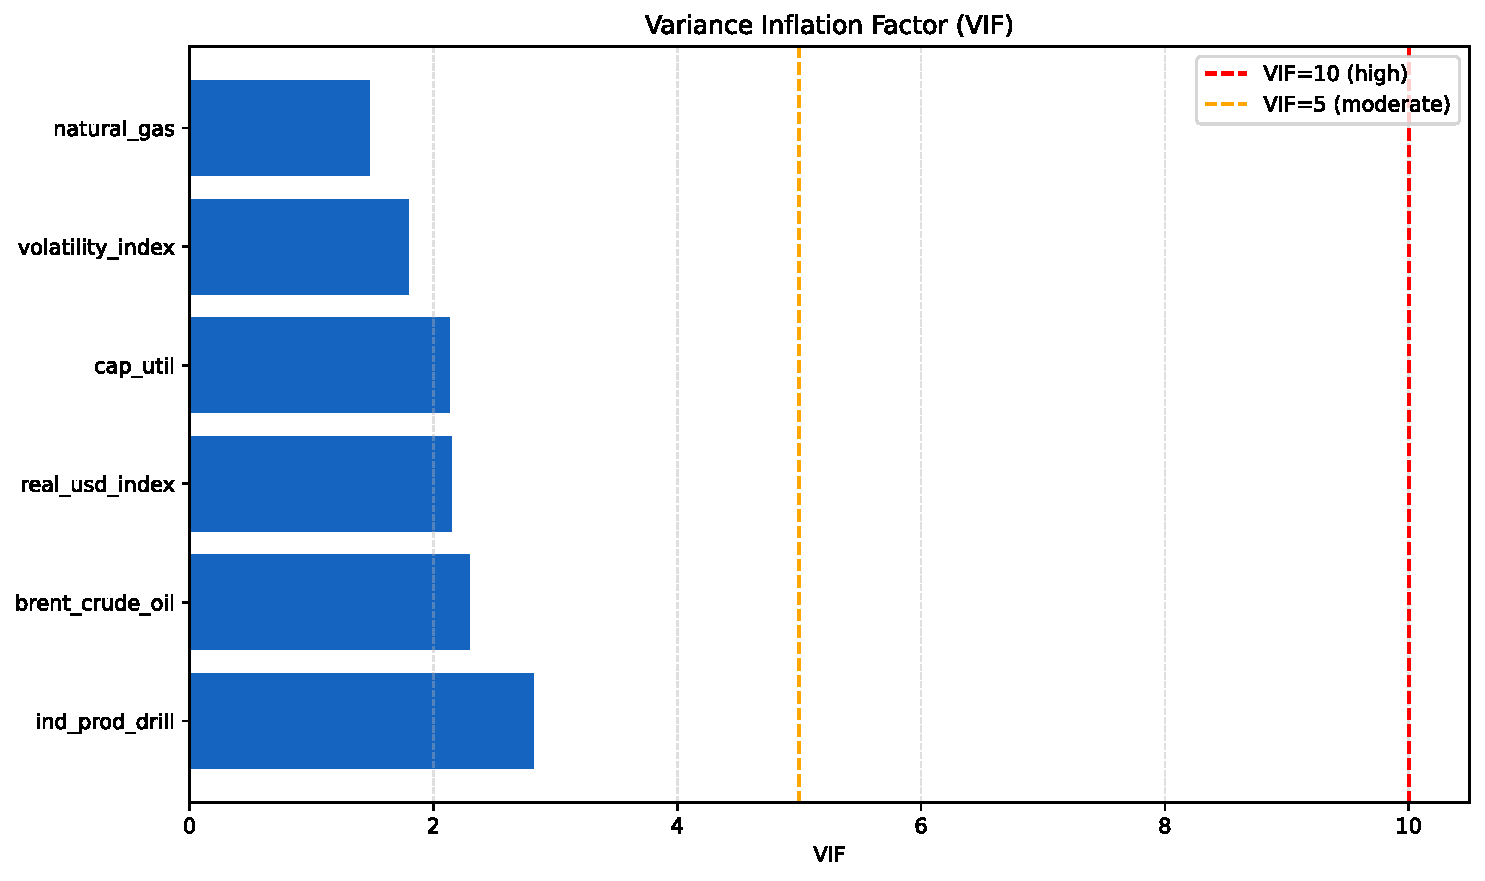
\includegraphics[width=0.85\linewidth]{vif_oil_macro_monthly_24_1_32.pdf}
\caption{Variance inflation factor table after pruning for the WTI monthly multivariate run with $w=24, h=1, b=32$. The retained regressors all satisfy $\mathrm{VIF} \le 10$.}\label{fig:vif}
\end{figure}

\begin{figure}[h!]
\centering
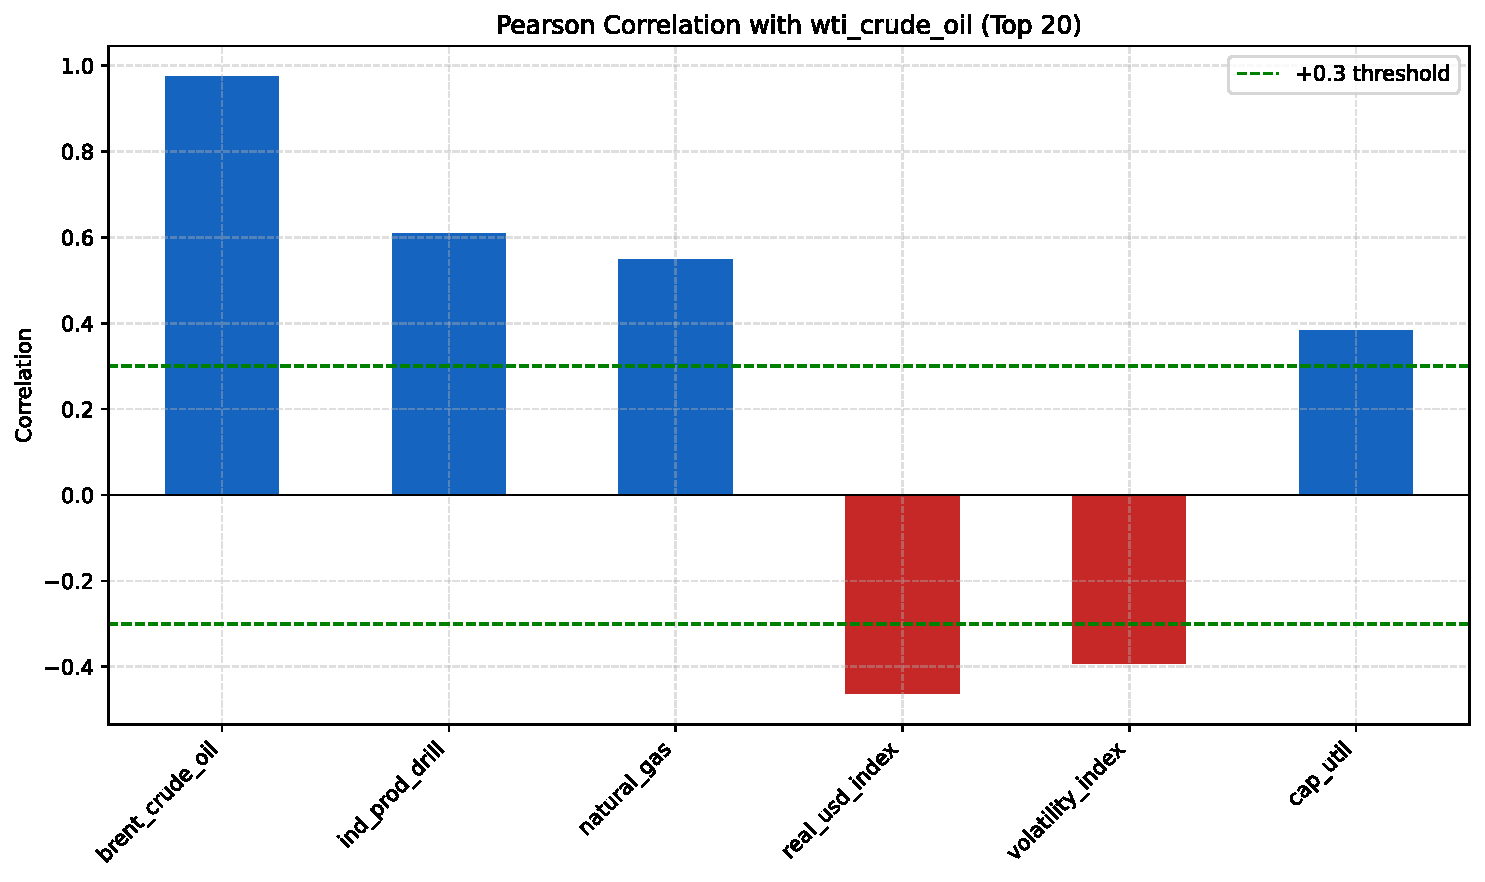
\includegraphics[width=0.95\linewidth]{pearson_oil_macro_monthly_24_1_32.pdf}
\caption{Pearson correlation matrix of the retained macro regressors for the WTI monthly multivariate run.}\label{fig:pearson}
\end{figure}

\paragraph{Evaluation metrics.}\label{sec:metrics}
All completed experiments are evaluated with mean squared error (MSE), root-mean-square error (RMSE), mean absolute error (MAE), mean absolute percentage error (MAPE\%), and the coefficient of determination $R^2$. Metrics are reported on train, test, and backtest slices where available. Statistical outputs are audited from stored CSV summaries, and neural outputs are audited from rendered metric panels. Figure~\ref{fig:arch} summarises the end-to-end architecture.

For an evaluation slice of length $n$, with actual price $y_t$, forecast $\hat{y}_t$, and sample mean $\bar{y}$, the reported metrics are
\begin{align}
\mathrm{MSE} &= \frac{1}{n}\sum_{t=1}^{n}(y_t-\hat{y}_t)^2, &
\mathrm{RMSE} &= \sqrt{\frac{1}{n}\sum_{t=1}^{n}(y_t-\hat{y}_t)^2}, \nonumber\\
\mathrm{MAE} &= \frac{1}{n}\sum_{t=1}^{n}|y_t-\hat{y}_t|, &
\mathrm{MAPE} &= \frac{100}{n}\sum_{t=1}^{n}\left|\frac{y_t-\hat{y}_t}{y_t}\right|, \label{eq:metrics}\\
R^2 &= 1-\frac{\sum_{t=1}^{n}(y_t-\hat{y}_t)^2}{\sum_{t=1}^{n}(y_t-\bar{y})^2}. \nonumber
\end{align}

\begin{figure}[h!]
\centering
\resizebox{\linewidth}{!}{%
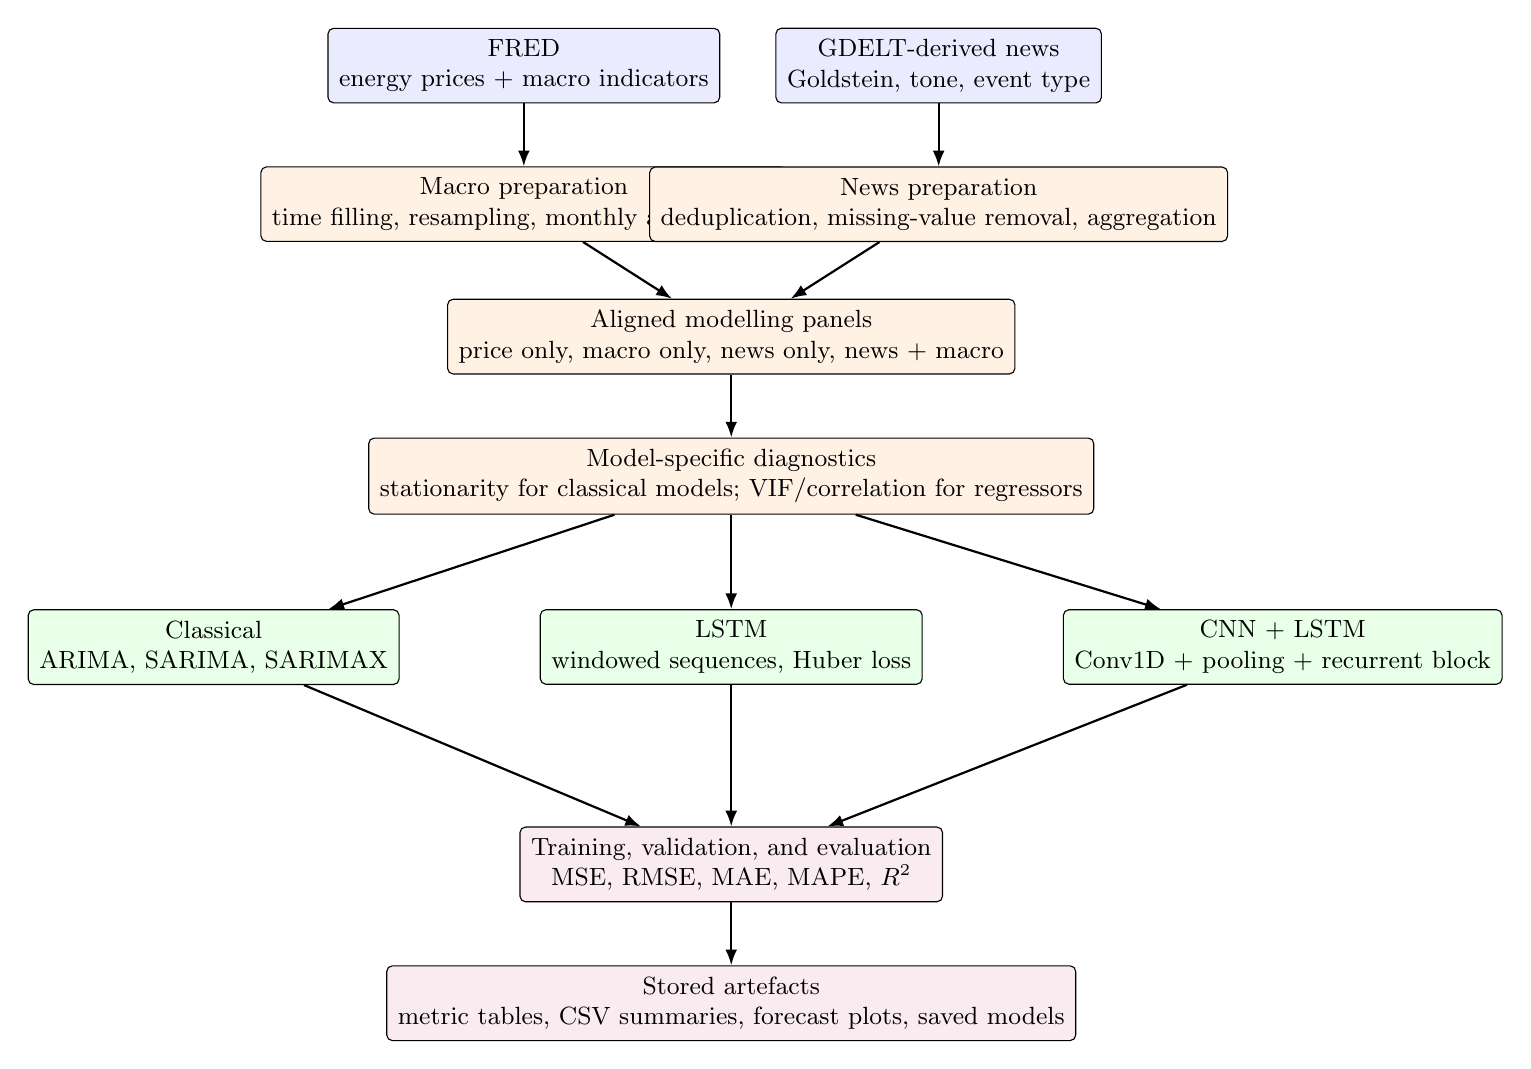
\begin{tikzpicture}[
  font=\small,
  node distance=8mm and 7mm,
  box/.style={draw, rounded corners=2pt, align=center, inner sep=4pt, minimum height=8mm},
  data/.style={box, fill=blue!8},
  prep/.style={box, fill=orange!10},
  model/.style={box, fill=green!9},
  eval/.style={box, fill=purple!8},
  arrow/.style={-{Latex[length=2mm]}, thick}
]
\node[data] (fred) {FRED\\energy prices + macro indicators};
\node[data, right=of fred] (gdelt) {GDELT-derived news\\Goldstein, tone, event type};
\node[prep, below=of fred] (macroprep) {Macro preparation\\time filling, resampling, monthly aggregation};
\node[prep, below=of gdelt] (newsprep) {News preparation\\deduplication, missing-value removal, aggregation};
\node[prep, below=12mm of $(macroprep)!0.5!(newsprep)$] (merge) {Aligned modelling panels\\price only, macro only, news only, news + macro};
\node[prep, below=of merge] (diag) {Model-specific diagnostics\\stationarity for classical models; VIF/correlation for regressors};
\node[model, below left=12mm and -4mm of diag] (classic) {Classical\\ARIMA, SARIMA, SARIMAX};
\node[model, below=12mm of diag] (lstm) {LSTM\\windowed sequences, Huber loss};
\node[model, below right=12mm and -4mm of diag] (cnnlstm) {CNN + LSTM\\Conv1D + pooling + recurrent block};
\node[eval, below=18mm of lstm] (evalnode) {Training, validation, and evaluation\\MSE, RMSE, MAE, MAPE, $R^2$};
\node[eval, below=of evalnode] (artifacts) {Stored artefacts\\metric tables, CSV summaries, forecast plots, saved models};
\draw[arrow] (fred) -- (macroprep);
\draw[arrow] (gdelt) -- (newsprep);
\draw[arrow] (macroprep) -- (merge);
\draw[arrow] (newsprep) -- (merge);
\draw[arrow] (merge) -- (diag);
\draw[arrow] (diag) -- (classic);
\draw[arrow] (diag) -- (lstm);
\draw[arrow] (diag) -- (cnnlstm);
\draw[arrow] (classic) -- (evalnode);
\draw[arrow] (lstm) -- (evalnode);
\draw[arrow] (cnnlstm) -- (evalnode);
\draw[arrow] (evalnode) -- (artifacts);
\end{tikzpicture}
}
\caption{Implemented project architecture. The diagram shows the public data sources, preparation pipeline, model groups, training and evaluation flow, and stored artefacts used in the paper.}\label{fig:arch}
\end{figure}

%%==================================================================%%
\section{Classical Time Series Models}\label{sec:classical}

The classical time-series stage includes price-only univariate baselines and multivariate models with exogenous regressors. Stationarity diagnostics are applied only within this classical modelling stage because differencing and order selection are specific to these models.

\paragraph{Stationarity testing.} Each relevant series is subjected to the Augmented Dickey-Fuller (ADF) test~\citep{dickey1979distribution} and the Kwiatkowski-Phillips-Schmidt-Shin (KPSS) test~\citep{kwiatkowski1992testing}. The two tests are complementary: the ADF rejects under stationarity, while the KPSS rejects under non-stationarity. When the tests indicate non-stationarity, differencing is applied and the tests are repeated until a stationary transformed series is obtained or the maximum differencing depth is reached.

\paragraph{Order selection.} Autocorrelation and partial autocorrelation diagnostics are used to nominate autoregressive and moving-average orders. Candidate orders are evaluated with information criteria and held-out metrics, and the reported values are taken only from completed stored outputs.

\begin{table}[h!]
\centering
\caption{Representative stationarity diagnostic for the differenced monthly WTI series. Values are transcribed from the stored stationarity panel.}\label{tab:stationarity}
\small
\begin{tabular}{@{}lrrl@{}}
\toprule
Test & Statistic & $p$-value & Verdict\\
\midrule
ADF  & $-10.2774$ & $0.0000$ & Stationary\\
KPSS & $0.0355$  & $0.1000$ & Stationary\\
\bottomrule
\end{tabular}
\end{table}

\paragraph{Seasonal decomposition.} Monthly series are decomposed into trend, seasonal, and residual components using additive seasonal decomposition with seasonal period twelve. A representative decomposition panel for the WTI monthly series is shown in Figure~\ref{fig:decomp}.

\begin{figure}[h!]
\centering
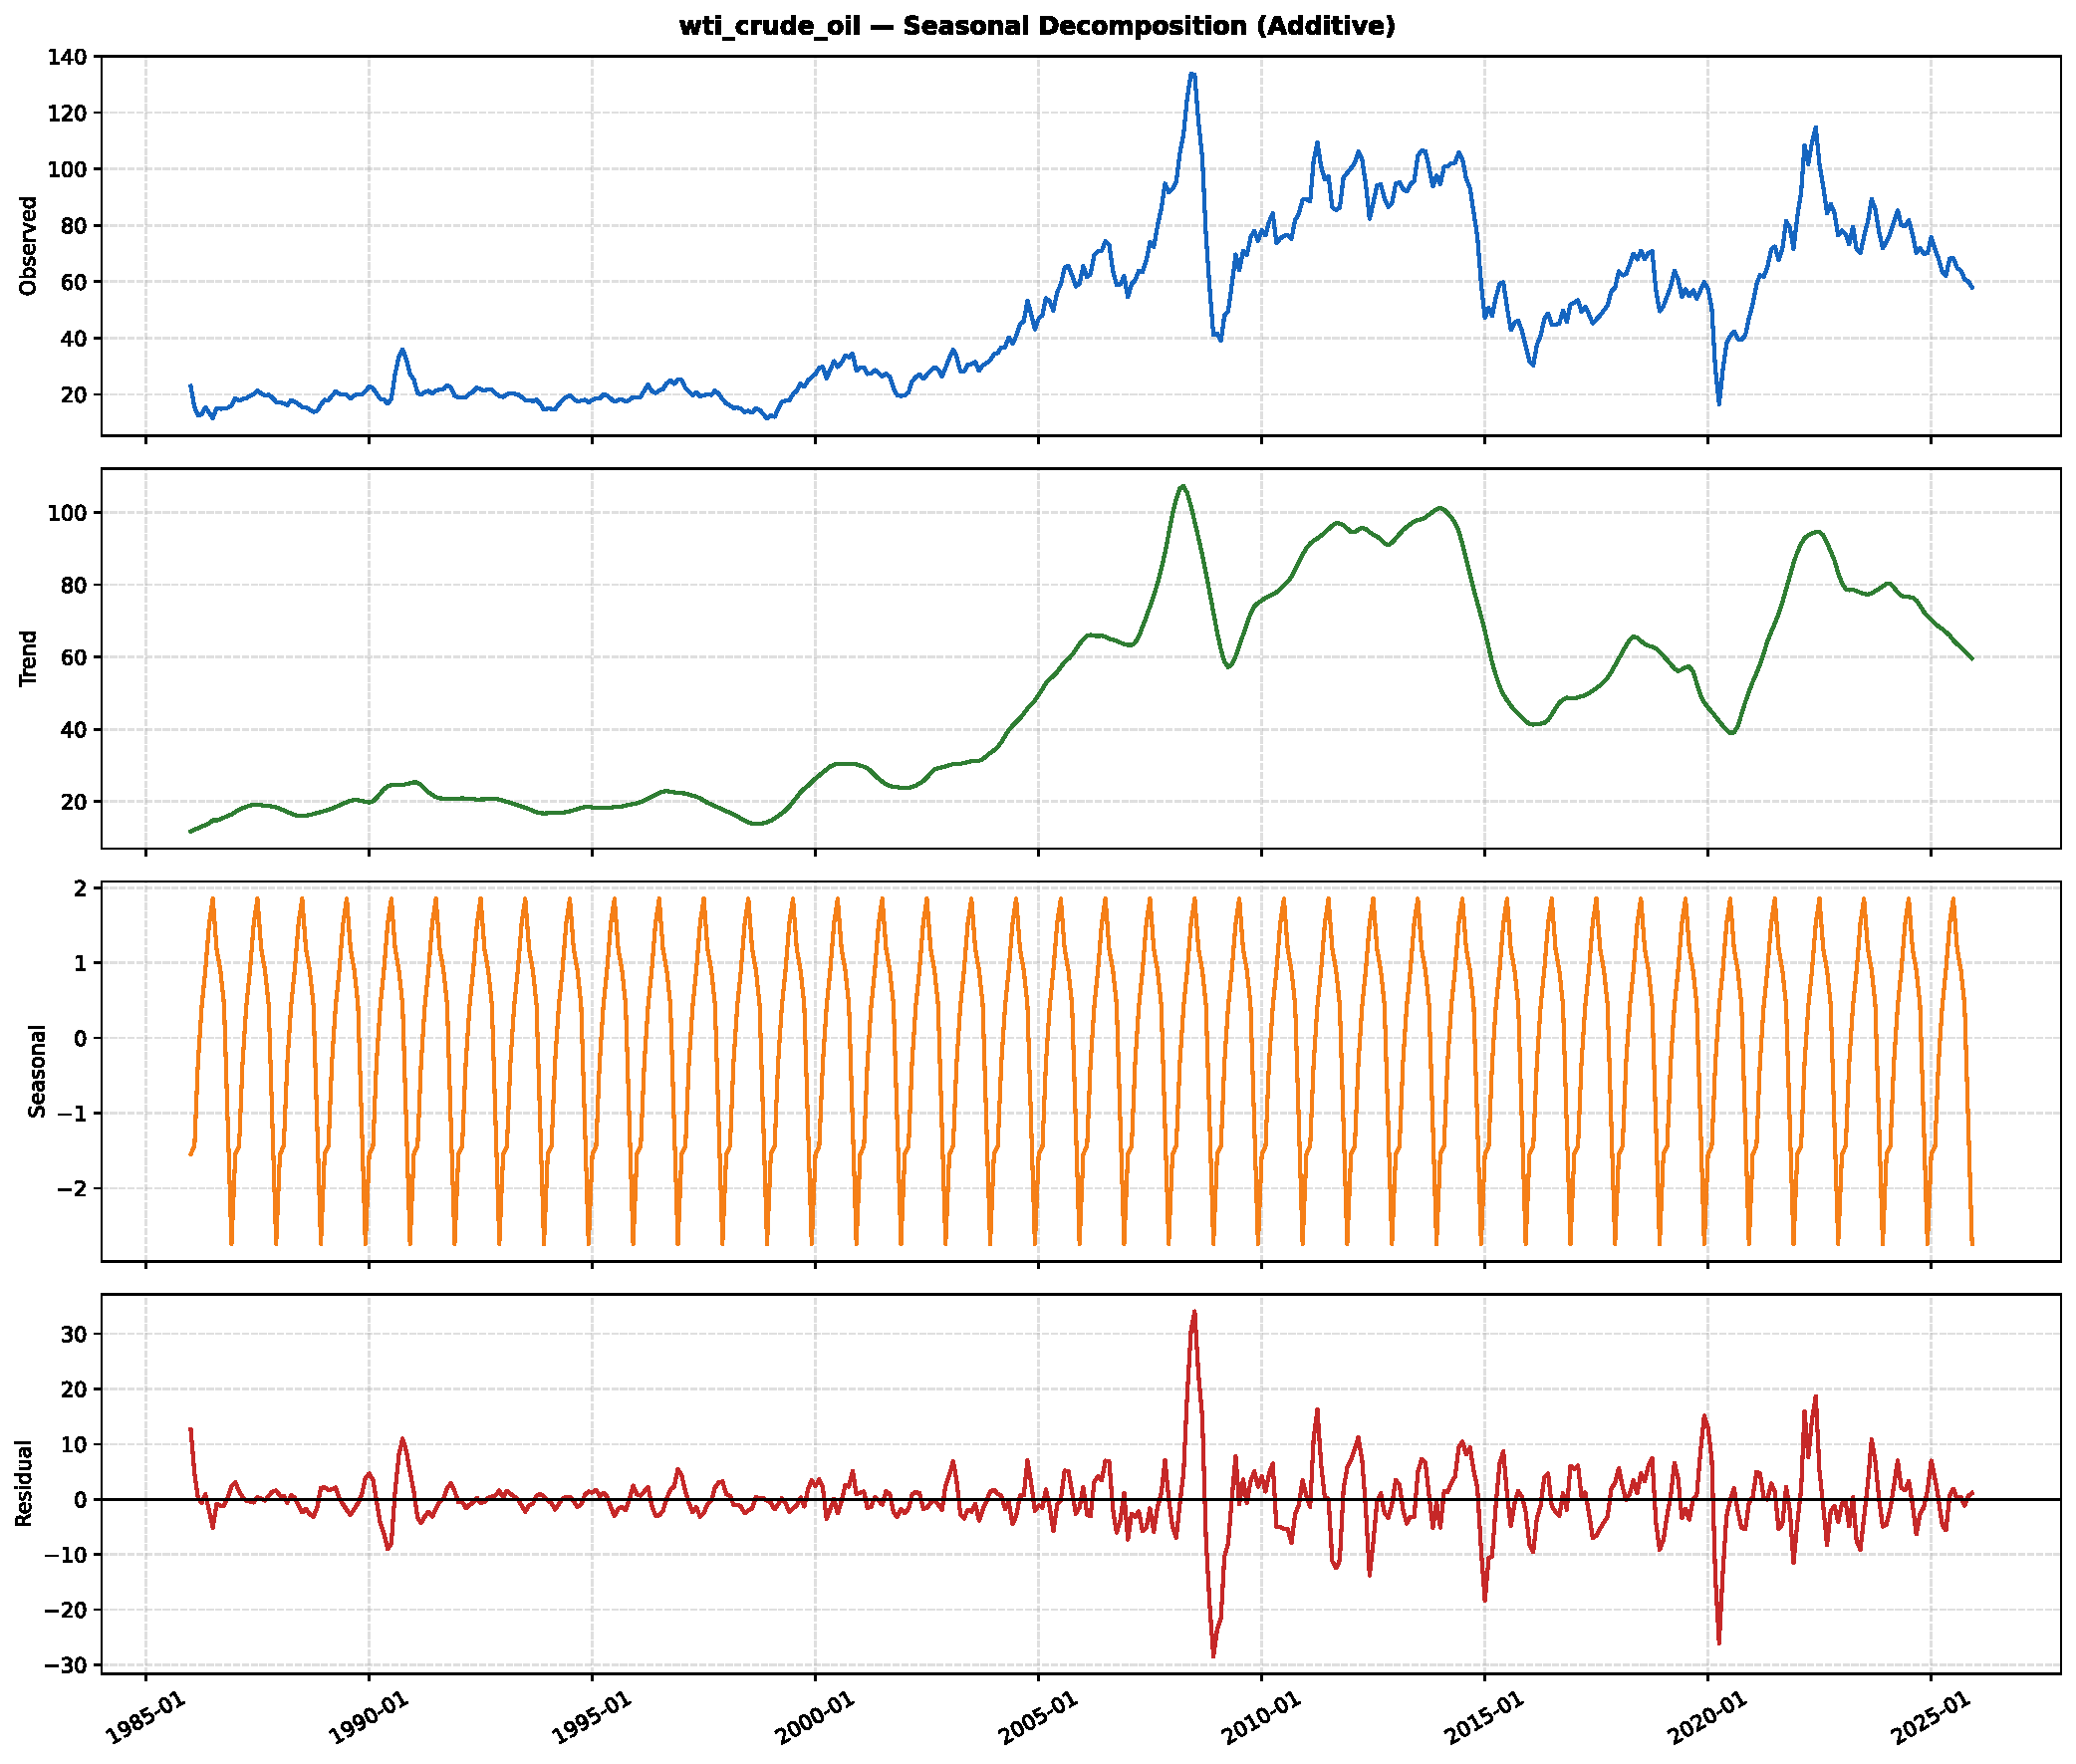
\includegraphics[width=0.95\linewidth]{oil_sarima_monthly_decomposition.pdf}
\caption{Additive seasonal decomposition of the monthly WTI series.}\label{fig:decomp}
\end{figure}

\subsection{Univariate baseline}

The univariate baseline uses only the historical price path. ARIMA is used for non-seasonal endogenous dynamics, while SARIMA adds a seasonal component for monthly or seasonally patterned series. These baselines provide a compact reference for interpreting the value of exogenous macroeconomic and news features.

Let $B$ denote the backshift operator, $\Delta^d=(1-B)^d$ the non-seasonal differencing operator, and $\varepsilon_t$ a white-noise innovation. The ARIMA formulation used for price-only non-seasonal baselines is
\begin{equation}
\phi(B)\Delta^d y_t = c + \theta(B)\varepsilon_t,
\label{eq:arima}
\end{equation}
where $\phi(B)=1-\phi_1B-\cdots-\phi_pB^p$ and $\theta(B)=1+\theta_1B+\cdots+\theta_qB^q$.

For seasonal price-only baselines, SARIMA adds the seasonal autoregressive and moving-average polynomials $\Phi(B^s)$ and $\Theta(B^s)$ with seasonal period $s$:
\begin{equation}
\Phi(B^s)\phi(B)(1-B)^d(1-B^s)^D y_t
= c + \Theta(B^s)\theta(B)\varepsilon_t.
\label{eq:sarima}
\end{equation}

\subsection{Multivariate}

SARIMAX extends the classical framework by adding an exogenous regressor matrix. In this study, SARIMAX is evaluated for macro-only and news-plus-macro input settings where completed metric outputs are available. The seasonal period is set to twelve for monthly experiments and is chosen from stored daily diagnostic outputs for daily experiments.

With exogenous feature vector $\mathbf{x}_t$ and coefficient vector $\boldsymbol{\beta}$, the SARIMAX form used for multivariate classical experiments is
\begin{equation}
\Phi(B^s)\phi(B)(1-B)^d(1-B^s)^D y_t
= c + \boldsymbol{\beta}^{\top}\mathbf{x}_t + \Theta(B^s)\theta(B)\varepsilon_t.
\label{eq:sarimax}
\end{equation}

%%==================================================================%%
\section{Neural Network Models}\label{sec:neural}

\subsection{Univariate}

The univariate neural model is an LSTM trained on a single-feature sequence of the target price. Completed univariate LSTM outputs are available for monthly WTI crude oil and monthly Henry Hub natural gas with input window $w=5$, output horizon $h=1$, and batch size $b=32$.

For an input sequence $\mathbf{x}_t$, the LSTM cell updates input, forget, candidate, and output gates as
\begin{align}
\mathbf{i}_t &= \sigma(W_i\mathbf{x}_t+U_i\mathbf{h}_{t-1}+\mathbf{b}_i), &
\mathbf{f}_t &= \sigma(W_f\mathbf{x}_t+U_f\mathbf{h}_{t-1}+\mathbf{b}_f), \nonumber\\
\tilde{\mathbf{c}}_t &= \tanh(W_c\mathbf{x}_t+U_c\mathbf{h}_{t-1}+\mathbf{b}_c), &
\mathbf{o}_t &= \sigma(W_o\mathbf{x}_t+U_o\mathbf{h}_{t-1}+\mathbf{b}_o), \label{eq:lstm-gates}\\
\mathbf{c}_t &= \mathbf{f}_t\odot\mathbf{c}_{t-1}+\mathbf{i}_t\odot\tilde{\mathbf{c}}_t, &
\mathbf{h}_t &= \mathbf{o}_t\odot\tanh(\mathbf{c}_t). \nonumber
\end{align}
The forecast head maps the final hidden representation to the horizon-specific prediction $\hat{\mathbf{y}}_{t+1:t+h}$.

\subsection{Multivariate}

The multivariate neural models use exogenous macroeconomic and/or GDELT-derived news features in addition to the target history. The LSTM configuration uses stacked recurrent layers followed by a dense projection and a linear forecast head. The CNN + LSTM configuration prepends a one-dimensional convolution and pooling step before the recurrent block, following the convolutional-recurrent design used in sequence modelling~\citep{sainath2015convolutional, lecun1998gradient}.

For the CNN + LSTM configuration, the one-dimensional convolution transforms a windowed feature sequence into local temporal filters before the recurrent block:
\begin{equation}
\mathbf{z}_{t,k} = g\!\left(b_k+\sum_{j=0}^{K-1} W_{k,j}^{\top}\mathbf{x}_{t+j}\right),
\label{eq:conv1d}
\end{equation}
where $K$ is the kernel width, $k$ indexes the filter, and $g(\cdot)$ is the nonlinear activation. The pooled convolutional sequence is then passed through the LSTM update in Equation~\eqref{eq:lstm-gates}.

\paragraph{Training setup.} Neural models are trained with the Adam optimiser~\citep{kingma2015adam} on Huber loss~\citep{huber1964robust}. Early stopping and learning-rate reduction are used to stabilise training. Hyperparameters are tuned with Optuna~\citep{akiba2019optuna}; completed leaves use the repository convention $(w,h,b)$ for input window, output horizon, and batch size.

Given residual $e_t=y_t-\hat{y}_t$, the Huber objective used for neural training is
\begin{equation}
\mathcal{L}_{\delta}(e_t)=
\begin{cases}
\frac{1}{2}e_t^2, & |e_t|\le \delta,\\
\delta\left(|e_t|-\frac{1}{2}\delta\right), & |e_t|>\delta.
\end{cases}
\label{eq:huber}
\end{equation}

%%==================================================================%%
\section{Results}\label{sec:results}

This section reports only completed configurations with stored metric artifacts. The discussion emphasises whether each configuration captures fluctuations clearly and whether the forecast path is stable across the held-out slice. The tables report test-slice RMSE, MAE, MAPE\%, and $R^2$ exactly as stored in the repository artifacts.

\subsection{Univariate models}\label{sec:res-uni}

For WTI crude oil, the monthly ARIMA output provides a usable medium-frequency baseline, the daily SARIMA output captures short-horizon fluctuations clearly, and the monthly LSTM output provides a neural price-only reference. For Henry Hub natural gas, the monthly ARIMA and monthly SARIMA outputs show stable monthly forecasting behaviour, while the univariate LSTM with $(w,h)=(5,1)$ provides the completed neural baseline. The selected univariate results are shown in Table~\ref{tab:uni-results}.

The univariate results are intentionally interpreted as baselines rather than as complete forecasting systems. Their value is that they isolate the information contained in the target series itself. When a univariate configuration is stable, the behaviour suggests that the commodity's own lagged movement contains enough persistence or seasonality for short-horizon forecasting. When it is unstable, the result indicates that price history alone is not sufficient for the held-out slice and that exogenous information may be needed to describe the observed movement.

\begin{table}[h!]
\centering
\caption{Selected univariate model outputs. Configurations are reported only where stored metrics are available.}\label{tab:uni-results}
\small
\resizebox{\linewidth}{!}{%
\begin{tabular}{@{}llllrrrr@{}}
\toprule
Commodity & Freq. & Model & Configuration & RMSE & MAE & MAPE\% & $R^2$ \\
\midrule
Oil & M & ARIMA  & $(0,1,1)$ & 6.832 & 6.343 & 10.494 & $-6.242$ \\
Oil & D & SARIMA & $(1,1,0)\!\times\!(0,1,0,12)$ & 1.210 & 1.081 & 1.868 & $-1.955$ \\
Oil & M & LSTM   & $(5,1,32)$ & 16.176 & 10.683 & 18.055 & $-39.589$ \\
CNG & M & ARIMA  & $(0,1,0)$ & 0.541 & 0.447 & 12.256 & $-0.139$ \\
CNG & M & SARIMA & $(0,1,0)\!\times\!(0,1,0,12)$ & 0.376 & 0.310 & 9.339 & $+0.449$ \\
CNG & M & LSTM   & $(5,1,32)$ & 0.554 & 0.497 & 14.721 & $-0.194$ \\
\bottomrule
\end{tabular}
}
\end{table}

\begin{figure}[h!]
\centering
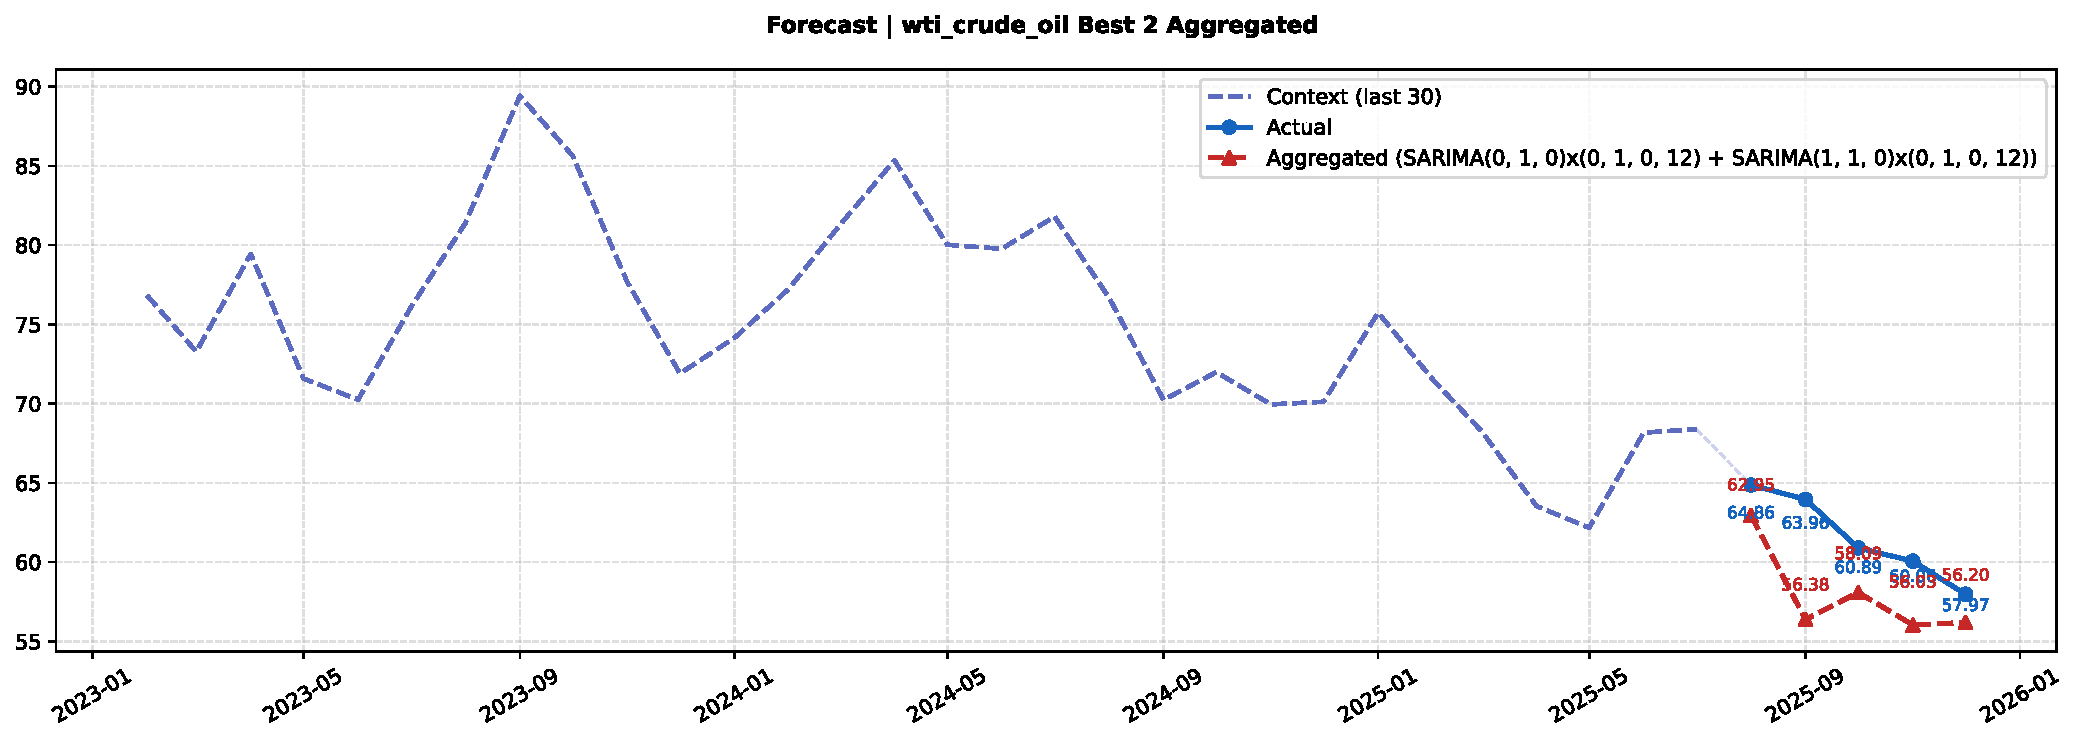
\includegraphics[width=0.85\linewidth]{oil_sarima_monthly_aggregated_forecast.pdf}
\caption{Two-order aggregated SARIMA forecast on the WTI monthly test block versus the actual price path.}\label{fig:uni-oil-forecast}
\end{figure}

\subsection{Multivariate models}\label{sec:res-multi}

The multivariate experiments evaluate macro-only, news-only, and news-plus-macro inputs. Table~\ref{tab:oil-multi} reports the selected WTI configurations. The macro CNN + LSTM run with $(w,h)=(36,1)$ produces a smooth monthly forecast path. The news-only CNN + LSTM run with $(w,h)=(24,5)$ captures medium-run movement but remains sensitive to the compressed news signal. In the fused news-plus-macro setting, the daily SARIMAX output captures daily fluctuations clearly, while the LSTM $(24,5)$ and CNN + LSTM $(36,5)$ outputs show stable multi-step monthly behaviour.

\begin{table}[h!]
\centering
\caption{Selected multivariate outputs for WTI crude oil.}\label{tab:oil-multi}
\small
\resizebox{\linewidth}{!}{%
\begin{tabular}{@{}llllrrrr@{}}
\toprule
Input set & Freq. & Model & Configuration & RMSE & MAE & MAPE\% & $R^2$ \\
\midrule
Macro & M & CNN + LSTM & $(36,1,32)$ & 8.342 & 7.008 & 11.763 & $-13.837$ \\
News only & M & CNN + LSTM & $(24,5,32)$ & 6.648 & 4.605 & 7.803 & $-8.711$ \\
News $+$ Macro & D & SARIMAX & $(0,1,1)\!\times\!(0,1,0,9)$ & 1.235 & 1.109 & 1.681 & $-2.166$ \\
News $+$ Macro & M & LSTM & $(24,5,32)$ & 2.921 & 2.378 & 4.011 & $-0.875$ \\
News $+$ Macro & M & CNN + LSTM & $(36,5,32)$ & 5.730 & 5.060 & 8.234 & $-6.214$ \\
\bottomrule
\end{tabular}
}
\end{table}

Table~\ref{tab:cng-multi} reports the selected Henry Hub natural gas configurations. The macro LSTM $(36,1)$ and macro CNN + LSTM $(36,1)$ outputs show consistent one-step monthly forecasting behaviour. The news-only CNN + LSTM $(36,1)$ output reflects the difficulty of using the news block alone for natural gas. In the fused setting, the LSTM $(36,5)$ and CNN + LSTM $(36,5)$ outputs capture monthly fluctuation patterns, while the daily SARIMAX output tracks short-horizon changes with small absolute error.

The multivariate tables should be read together with the forecast plots rather than as isolated scoreboards. A configuration can have a larger RMSE because it misses the level of the target while still following the direction of movement; conversely, a low error on a short and smooth test slice may not imply broad robustness. For this reason, the paper reports RMSE, MAE, MAPE, and $R^2$ together and includes representative forecast figures for the news-plus-macro setting.

\begin{table}[h!]
\centering
\caption{Selected multivariate outputs for Henry Hub natural gas.}\label{tab:cng-multi}
\small
\resizebox{\linewidth}{!}{%
\begin{tabular}{@{}llllrrrr@{}}
\toprule
Input set & Freq. & Model & Configuration & RMSE & MAE & MAPE\% & $R^2$ \\
\midrule
Macro & M & LSTM & $(36,1,32)$ & 1.526 & 1.227 & 26.348 & $+0.215$ \\
Macro & M & CNN + LSTM & $(36,1,32)$ & 1.801 & 1.313 & 25.897 & $-0.093$ \\
News only & M & CNN + LSTM & $(36,1,32)$ & 4.357 & 3.932 & 107.173 & $-5.412$ \\
News $+$ Macro & M & LSTM & $(36,5,32)$ & 1.727 & 1.501 & 33.432 & $-0.008$ \\
News $+$ Macro & M & CNN + LSTM & $(36,5,32)$ & 1.153 & 0.943 & 22.204 & $+0.550$ \\
News $+$ Macro & D & SARIMAX & $(0,1,1)\!\times\!(0,1,0,6)$ & 0.087 & 0.080 & 2.661 & $-0.879$ \\
\bottomrule
\end{tabular}
}
\end{table}

Figures~\ref{fig:oil-selected} and~\ref{fig:cng-selected} provide representative forecast panels for the news-plus-macro setting. The WTI LSTM $(24,5)$ panel shows a coherent five-step trajectory and a close train-validation loss pattern. The Henry Hub CNN + LSTM $(36,5)$ panel shows stable monthly movement on the test horizon and provides an additional backtest view.

\begin{figure}[h!]
\centering
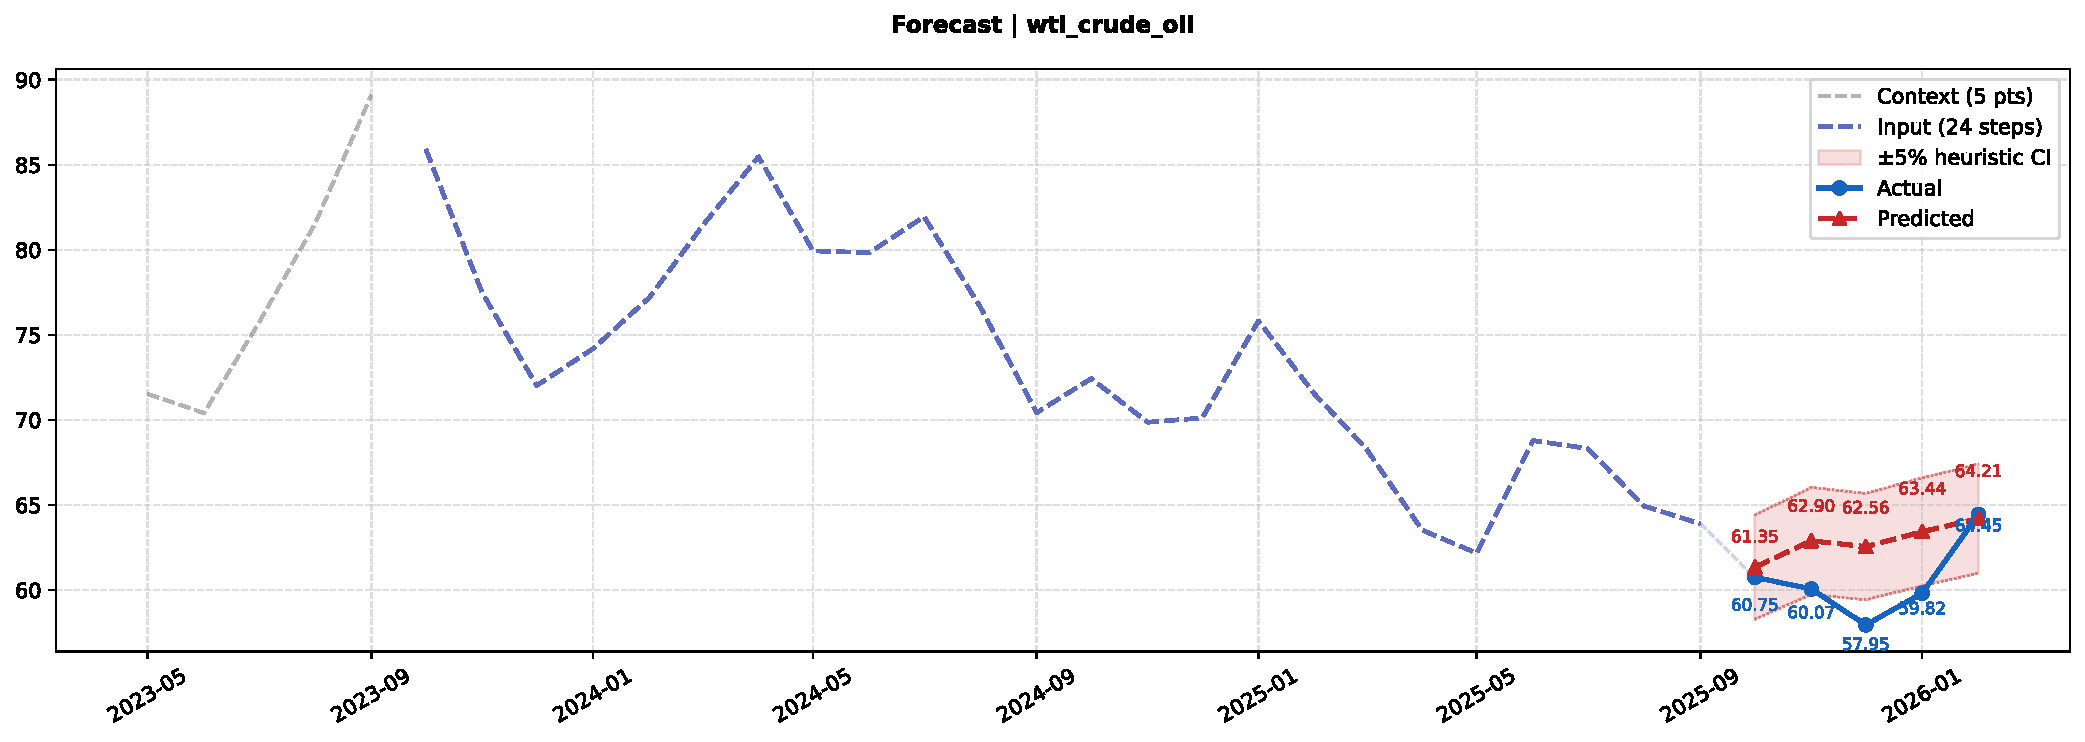
\includegraphics[width=0.49\linewidth]{oil_news_macro_lstm_24_5_32_forecast.pdf}\hfill
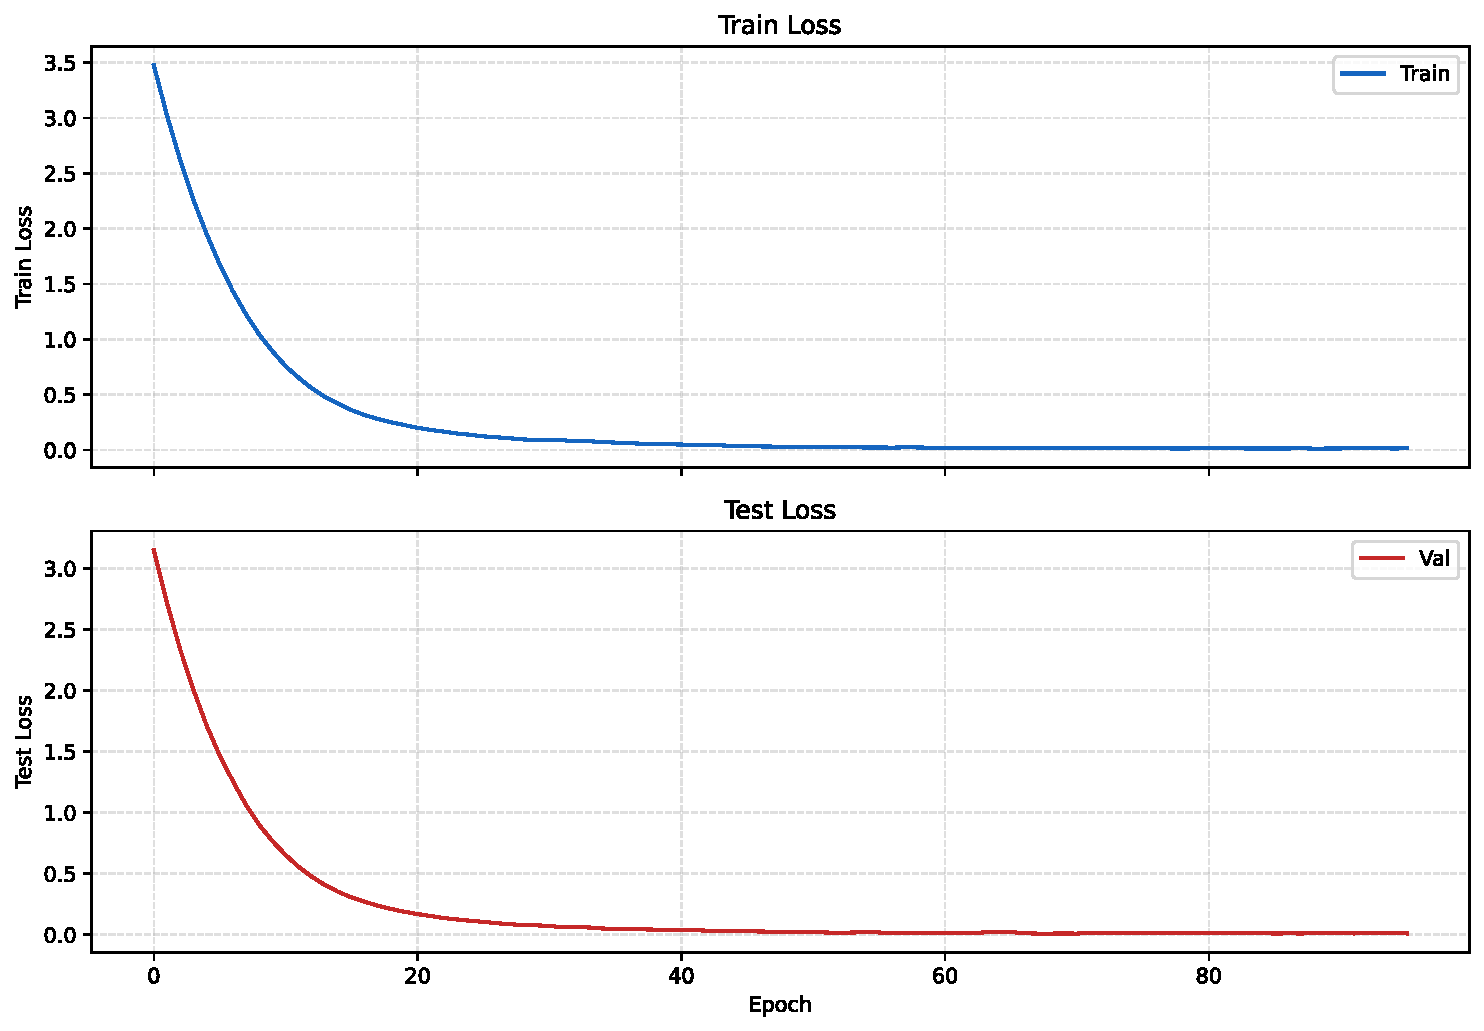
\includegraphics[width=0.49\linewidth]{oil_news_macro_lstm_24_5_32_loss.pdf}
\caption{WTI monthly LSTM trained on news-plus-macro inputs with $w=24, h=5, b=32$. Left: forecast on the five-step held-out horizon. Right: training and validation loss curves.}\label{fig:oil-selected}
\end{figure}

\begin{figure}[h!]
\centering
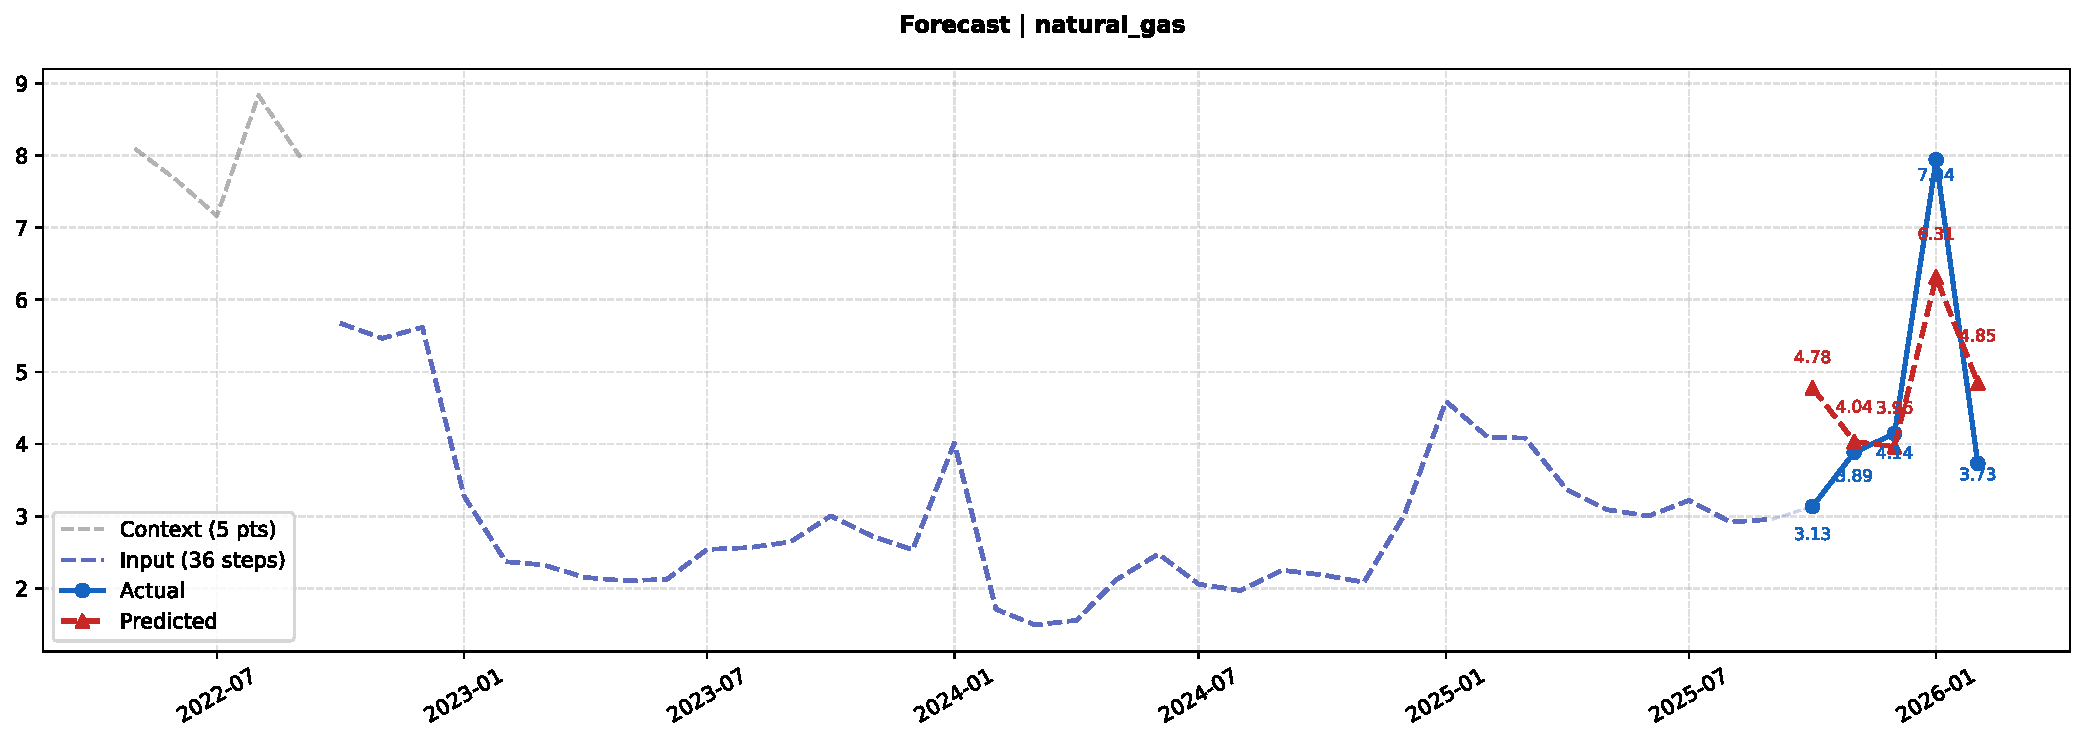
\includegraphics[width=0.49\linewidth]{cng_news_macro_cnn_lstm_36_5_32_forecast.pdf}\hfill
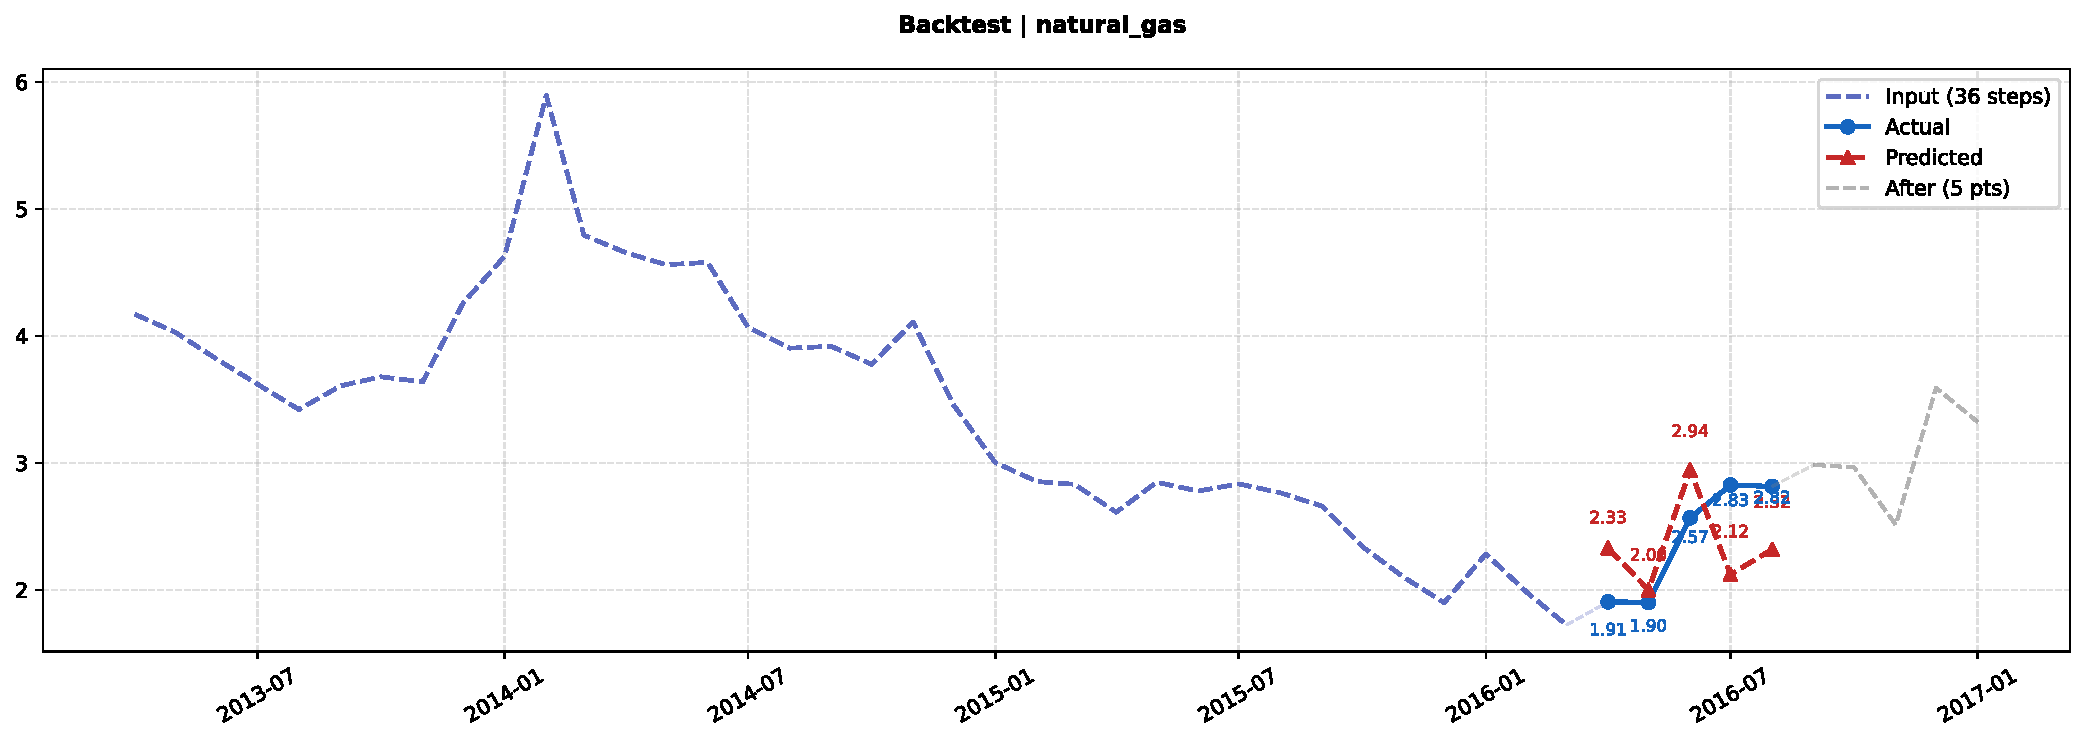
\includegraphics[width=0.49\linewidth]{cng_news_macro_cnn_lstm_36_5_32_backtest.pdf}
\caption{Henry Hub monthly CNN + LSTM trained on news-plus-macro inputs with $w=36, h=5, b=32$. Left: forecast on the test horizon. Right: backtest panel.}\label{fig:cng-selected}
\end{figure}

%%==================================================================%%
\section{Discussion}\label{sec:discussion}

The GDELT-derived news block contributes most clearly when it is fused with macroeconomic variables rather than used as a standalone signal. On WTI monthly, the news-plus-macro LSTM $(24,5)$ output produces a coherent five-step path, and on Henry Hub monthly the news-plus-macro CNN + LSTM $(36,5)$ output follows the direction of the held-out movement with stable backtest behaviour. On WTI daily, the news-plus-macro SARIMAX output captures short-horizon fluctuations with low absolute error.

A plausible interpretation is that the news block functions as a slow-moving regime variable. Its informational content is easier to observe at the monthly horizon, where the persistent direction of policy and macroeconomic narrative reporting can be aggregated into a meaningful exogenous signal. At daily frequency, the same block is more sensitive to short-horizon noise, and stable behaviour appears only when the model structure and differencing procedure dampen that noise.

The commodity difference is also important. WTI crude oil is heavily exposed to broad macro-financial and geopolitical narratives, so a news-plus-macro representation has a clearer interpretation in the monthly WTI experiments. Henry Hub natural gas, by contrast, often responds to regional demand, storage, and weather-related pressures that are not fully captured by the current feature set. This helps explain why the natural-gas results should be read cautiously even when the numerical test error is small.

\subsection{Classical and neural behaviour}

The classical outputs remain informative because they require relatively few parameters and respond directly to stationarity and seasonal structure. The neural outputs become more useful when longer windows and fused exogenous inputs are available, especially in monthly settings where the signal is less noisy than daily movement. This pattern is consistent with the training data constraint: recurrent models require enough contiguous sequences to learn stable dynamics, while classical models can remain steady under shorter samples.

This distinction is methodological rather than philosophical. The classical models offer transparency through differencing, order selection, and explicit exogenous coefficients. The neural models offer flexibility through nonlinear sequence transformations, but the same flexibility can amplify noise when the training sample is short. In this project, the most interpretable neural outputs are therefore the configurations whose forecast plots show smooth movement and whose training curves do not separate sharply between training and validation loss.

\subsection{Hyperparameter sensitivity}

Across the neural leaves, test RMSE is non-monotonic in the input window. Longer windows provide more historical context, but they also reduce the number of admissible training sequences. The stored outputs therefore suggest a practical trade-off: windows such as $(24,5)$ and $(36,5)$ can capture multi-step movement, while very long windows may compress the effective training set too severely for stable generalisation.

The WTI monthly news-plus-macro LSTM illustrates this trade-off. Its $(24,5)$ configuration produces a coherent five-step trajectory, suggesting that direct multi-step forecasting can act as a regularising constraint by requiring the model to learn a short path rather than a single isolated point.

%%==================================================================%%
\section{Limitations}\label{sec:limits}

The study is subject to four limitations. First, the public macroeconomic and news-derived datasets have different native frequencies and reporting calendars, so alignment and aggregation may smooth or delay parts of the signal. Second, the test windows are finite and should be interpreted as held-out point estimates rather than full uncertainty intervals. Third, the models remain sensitive to external events such as geopolitical shocks, weather disruptions, policy changes, and sudden demand shifts that may not be fully represented by the available features. Fourth, only configurations with complete stored metric artifacts are included in the tables; this protects reproducibility but limits the breadth of the comparison.

A further practical limitation is that the available news representation is event-level and numeric. It does not preserve full article text, source identity, or topic-level nuance beyond the retained GDELT-derived fields. The design is therefore appropriate for a reproducible tabular forecasting study, but it cannot answer finer questions about which individual stories, countries, or narrative themes drove a particular forecast movement.

%%==================================================================%%
\section{Future Work}\label{sec:future-work}

Future work can extend the project in four directions. First, feature engineering can be improved by adding lagged macro variables, rolling volatility summaries, shock indicators, and richer transformations of the news features. Second, advanced deep learning architectures can be evaluated under the same walk-forward protocol once sufficient training data and stored artifacts are available. Third, the pipeline can be adapted for real-time forecasting so that new FRED releases and GDELT events update the feature panel automatically. Fourth, additional external data sources, including weather variables, shipping indicators, inventory reports, and geopolitical-event datasets, can be integrated to capture drivers that are not fully represented in the current input blocks.

%%==================================================================%%
\section{Conclusion}\label{sec:conclusion}

This work presents a reproducible comparison of univariate and multivariate forecasting approaches for WTI crude oil and Henry Hub natural gas prices. The results show that price-only monthly baselines can capture stable seasonal movement, that exogenous macroeconomic inputs provide useful context, and that GDELT-derived news signals are most interpretable when fused with macroeconomic variables. The stored outputs also show that forecasting behaviour differs across commodity and frequency: daily experiments are sensitive to short-horizon noise, while monthly experiments make longer-window configurations easier to interpret. Every numerical claim in this paper is traceable to a stored CSV table or rendered metric panel in the project repository.

%%==================================================================%%
\section{Reproducibility}\label{sec:reproducibility}

The repository preserves the data inputs, metric tables, forecast plots, diagnostic figures, and saved model artifacts needed to audit the reported values. Statistical results are read from stored CSV summaries, while neural results are read from rendered metric panels. Each number in the Results section can therefore be traced to a corresponding artifact in the results directory. Configurations without complete stored metric artifacts are not reported in the tables, which preserves factual correctness and avoids unverifiable claims.

\backmatter

\bmhead{Supplementary information}
The full set of metric tables, forecast plots, EDA panels, and saved model files is provided in the \texttt{results/} subtree of the repository. Additional hyperparameter sweeps are retained in the same subtree for completeness.

\bmhead{Acknowledgements}
The authors thank the maintainers of FRED and GDELT for the public data infrastructure on which this work depends. This work was carried out as part of the Data Science Capstone Program at The George Washington University.

\section*{Declarations}

\noindent\textbf{Funding.} This work received no external funding.\\
\textbf{Conflict of interest.} The authors declare no competing interests.\\
\textbf{Data availability.} All data are obtained from public APIs (FRED and GDELT). The macro series identifiers are listed in Table~\ref{tab:fred-series}.\\
\textbf{Project availability.} The full project repository is publicly available at \url{https://github.com/AswinBalajiTR/spring-2026-group6}.\\
\textbf{Author contribution.} Aswin Balaji Thippa Ramesh and Vishal Balaji Fulsundar designed the experiments, implemented the experimental workflow, and ran the analyses. Amir Hossein Jafari supervised the work. All authors contributed to writing the manuscript.

%%==================================================================%%
\bibliographystyle{plainnat}%
\begin{thebibliography}{99}

\bibitem[Akaike(1974)]{akaike1974new}
Akaike, H.: A new look at the statistical model identification. \emph{IEEE Transactions on Automatic Control} \textbf{19}(6), 716--723 (1974).

\bibitem[Akiba et al.(2019)]{akiba2019optuna}
Akiba, T., Sano, S., Yanase, T., Ohta, T., Koyama, M.: Optuna: A next-generation hyperparameter optimization framework. In: \emph{Proceedings of the 25th ACM SIGKDD International Conference on Knowledge Discovery and Data Mining}, pp.\ 2623--2631 (2019).

\bibitem[Baker et al.(2016)]{baker2016measuring}
Baker, S.R., Bloom, N., Davis, S.J.: Measuring economic policy uncertainty. \emph{The Quarterly Journal of Economics} \textbf{131}(4), 1593--1636 (2016).

\bibitem[Baumeister and Kilian(2016)]{baumeister2016forty}
Baumeister, C., Kilian, L.: Forty years of oil price fluctuations: why the price of oil may still surprise us. \emph{Journal of Economic Perspectives} \textbf{30}(1), 139--160 (2016).

\bibitem[Box and Jenkins(1976)]{box1976time}
Box, G.E.P., Jenkins, G.M.: \emph{Time Series Analysis: Forecasting and Control}. Holden-Day, San Francisco (1976).

\bibitem[Busari and Lim(2021)]{busari2021crude}
Busari, G.A., Lim, D.H.: Crude oil price prediction: a comparison between AdaBoost-LSTM and AdaBoost-GRU for improving forecasting performance. \emph{Computers \& Chemical Engineering} \textbf{155}, 107513 (2021).

\bibitem[Cen and Wang(2019)]{cen2019crude}
Cen, Z., Wang, J.: Crude oil price prediction model with long short-term memory deep learning based on prior knowledge data transfer. \emph{Energy} \textbf{169}, 160--171 (2019).

\bibitem[Dickey and Fuller(1979)]{dickey1979distribution}
Dickey, D.A., Fuller, W.A.: Distribution of the estimators for autoregressive time series with a unit root. \emph{Journal of the American Statistical Association} \textbf{74}(366), 427--431 (1979).

\bibitem[Diebold and Mariano(1995)]{diebold1995comparing}
Diebold, F.X., Mariano, R.S.: Comparing predictive accuracy. \emph{Journal of Business \& Economic Statistics} \textbf{13}(3), 253--263 (1995).

\bibitem[Durbin and Koopman(2012)]{durbin2012time}
Durbin, J., Koopman, S.J.: \emph{Time Series Analysis by State Space Methods}, 2nd edn. Oxford University Press, Oxford (2012).

\bibitem[Federal Reserve(2024)]{fred2024}
Federal Reserve Bank of St.\ Louis: \emph{Federal Reserve Economic Data (FRED)}. \url{https://fred.stlouisfed.org/} (accessed 2025).

\bibitem[Gers et al.(2000)]{gers2000learning}
Gers, F.A., Schmidhuber, J., Cummins, F.: Learning to forget: continual prediction with LSTM. \emph{Neural Computation} \textbf{12}(10), 2451--2471 (2000).

\bibitem[Goldstein(1992)]{goldstein1992conflict}
Goldstein, J.S.: A conflict-cooperation scale for WEIS events data. \emph{Journal of Conflict Resolution} \textbf{36}(2), 369--385 (1992).

\bibitem[Hamilton(2003)]{hamilton2003what}
Hamilton, J.D.: What is an oil shock? \emph{Journal of Econometrics} \textbf{113}(2), 363--398 (2003).

\bibitem[Hamilton(2009)]{hamilton2009causes}
Hamilton, J.D.: Causes and consequences of the oil shock of 2007--08. \emph{Brookings Papers on Economic Activity} \textbf{2009}(1), 215--261 (2009).

\bibitem[Hochreiter and Schmidhuber(1997)]{hochreiter1997long}
Hochreiter, S., Schmidhuber, J.: Long short-term memory. \emph{Neural Computation} \textbf{9}(8), 1735--1780 (1997).

\bibitem[Huber(1964)]{huber1964robust}
Huber, P.J.: Robust estimation of a location parameter. \emph{Annals of Mathematical Statistics} \textbf{35}(1), 73--101 (1964).

\bibitem[Hyndman and Athanasopoulos(2018)]{hyndman2018forecasting}
Hyndman, R.J., Athanasopoulos, G.: \emph{Forecasting: Principles and Practice}, 2nd edn. OTexts, Melbourne (2018).

\bibitem[Kilian(2009)]{kilian2009not}
Kilian, L.: Not all oil price shocks are alike: disentangling demand and supply shocks in the crude oil market. \emph{American Economic Review} \textbf{99}(3), 1053--1069 (2009).

\bibitem[Kim and Won(2018)]{kim2019predicting}
Kim, H.Y., Won, C.H.: Forecasting the volatility of stock price index: a hybrid model integrating LSTM with multiple GARCH-type models. \emph{Expert Systems with Applications} \textbf{103}, 25--37 (2018).

\bibitem[Kingma and Ba(2015)]{kingma2015adam}
Kingma, D.P., Ba, J.: Adam: a method for stochastic optimization. In: \emph{International Conference on Learning Representations} (2015).

\bibitem[Kwiatkowski et al.(1992)]{kwiatkowski1992testing}
Kwiatkowski, D., Phillips, P.C.B., Schmidt, P., Shin, Y.: Testing the null hypothesis of stationarity against the alternative of a unit root. \emph{Journal of Econometrics} \textbf{54}(1--3), 159--178 (1992).

\bibitem[LeCun et al.(1998)]{lecun1998gradient}
LeCun, Y., Bottou, L., Bengio, Y., Haffner, P.: Gradient-based learning applied to document recognition. \emph{Proceedings of the IEEE} \textbf{86}(11), 2278--2324 (1998).

\bibitem[Leetaru and Schrodt(2013)]{leetaru2013gdelt}
Leetaru, K., Schrodt, P.A.: GDELT: Global Data on Events, Location, and Tone, 1979--2012. In: \emph{ISA Annual Convention} (2013).

\bibitem[Li et al.(2014)]{li2014news}
Li, X., Xie, H., Chen, L., Wang, J., Deng, X.: News impact on stock price return via sentiment analysis. \emph{Knowledge-Based Systems} \textbf{69}, 14--23 (2014).

\bibitem[Sainath et al.(2015)]{sainath2015convolutional}
Sainath, T.N., Vinyals, O., Senior, A., Sak, H.: Convolutional, long short-term memory, fully connected deep neural networks. In: \emph{Proceedings of the IEEE International Conference on Acoustics, Speech and Signal Processing (ICASSP)}, pp.\ 4580--4584 (2015).

\bibitem[Shapiro et al.(2022)]{shapiro2022measuring}
Shapiro, A.H., Sudhof, M., Wilson, D.J.: Measuring news sentiment. \emph{Journal of Econometrics} \textbf{228}(2), 221--243 (2022).

\bibitem[Tetlock(2007)]{tetlock2007giving}
Tetlock, P.C.: Giving content to investor sentiment: the role of media in the stock market. \emph{The Journal of Finance} \textbf{62}(3), 1139--1168 (2007).

\end{thebibliography}

%%==================================================================%%
\begin{appendices}

\section{Formula Reference and Notation}\label{app:formula-reference}

This appendix consolidates the notation used in the model and metric formulas. The symbol $y_t$ denotes the observed energy price at time $t$, $\hat{y}_t$ denotes the corresponding forecast, $\mathbf{x}_t$ denotes the exogenous feature vector, and $\varepsilon_t$ denotes the innovation term in the classical time-series models. The backshift operator is $B$, so that $By_t=y_{t-1}$. The non-seasonal orders are $(p,d,q)$ and the seasonal orders are $(P,D,Q,s)$, where $s$ is the seasonal period. For neural configurations, $(w,h,b)$ denotes input window length, forecast horizon, and batch size.

\begin{table}[h!]
\centering
\caption{Formula locations used in the manuscript.}\label{tab:formula-reference}
\small
\begin{tabular}{@{}lll@{}}
\toprule
Component & Equation & Purpose\\
\midrule
Evaluation metrics & Eq.~\eqref{eq:metrics} & MSE, RMSE, MAE, MAPE, and $R^2$ reporting\\
ARIMA & Eq.~\eqref{eq:arima} & Non-seasonal univariate baseline\\
SARIMA & Eq.~\eqref{eq:sarima} & Seasonal univariate baseline\\
SARIMAX & Eq.~\eqref{eq:sarimax} & Classical multivariate model with exogenous features\\
LSTM gates & Eq.~\eqref{eq:lstm-gates} & Recurrent sequence update\\
CNN + LSTM convolution & Eq.~\eqref{eq:conv1d} & Local temporal feature extraction before recurrence\\
Huber loss & Eq.~\eqref{eq:huber} & Neural training objective\\
\bottomrule
\end{tabular}
\end{table}

\section{Artifact Traceability}\label{app:artifact-traceability}

All numeric results reported in Tables~\ref{tab:uni-results},~\ref{tab:oil-multi}, and~\ref{tab:cng-multi} are copied from stored result artifacts. Classical metrics are taken from CSV summaries produced for the corresponding fitted orders. Neural metrics are taken from rendered metric panels in the relevant result folders. Forecast plots in Figures~\ref{fig:uni-oil-forecast},~\ref{fig:oil-selected}, and~\ref{fig:cng-selected} are reproduced from the stored forecast artifacts. This appendix is included to clarify that the equations describe the modelling and evaluation framework, while the reported numbers remain tied to completed repository outputs.

\begin{table}[h!]
\centering
\caption{Traceability map for the result tables.}\label{tab:artifact-map}
\small
\resizebox{\linewidth}{!}{%
\begin{tabular}{@{}llll@{}}
\toprule
Reported table & Commodity scope & Model scope & Artifact type used for auditing\\
\midrule
Table~\ref{tab:uni-results} & WTI and Henry Hub & Price-only classical and LSTM outputs & Stored statistical summaries and neural metric panels\\
Table~\ref{tab:oil-multi} & WTI crude oil & Macro, news-only, and news-plus-macro outputs & Stored metric panels and SARIMAX summary table\\
Table~\ref{tab:cng-multi} & Henry Hub natural gas & Macro, news-only, and news-plus-macro outputs & Stored metric panels and SARIMAX summary table\\
Figure~\ref{fig:uni-oil-forecast} & WTI crude oil & Price-only seasonal baseline & Stored forecast plot\\
Figures~\ref{fig:oil-selected}--\ref{fig:cng-selected} & WTI and Henry Hub & News-plus-macro neural outputs & Stored forecast, loss, and backtest plots\\
\bottomrule
\end{tabular}
}
\end{table}

\section{Reading the Reported Metrics}\label{app:metric-reading}

RMSE and MAE are reported in the same units as the target price, so they are the most direct indicators of average forecast error. MAPE is unit-free and useful for comparing across commodities, but it can become unstable when the actual price level is small. The $R^2$ values in short held-out windows should be interpreted carefully: a negative value does not necessarily mean that the forecast is visually useless; it can also occur when the test slice has low variance and a small level error is large relative to that variance. For this reason, the paper pairs the tables with forecast plots and avoids relying on a single metric alone.

\begin{table}[h!]
\centering
\caption{Interpretation guide for the reported evaluation metrics.}\label{tab:metric-guide}
\small
\resizebox{\linewidth}{!}{%
\begin{tabular}{@{}lll@{}}
\toprule
Metric & Scale & Interpretation in this study\\
\midrule
RMSE & Target-price units & Penalises large point errors and is used for compact comparison\\
MAE & Target-price units & Reports average absolute deviation from the held-out path\\
MAPE & Percent & Provides a relative error view across oil and natural gas\\
$R^2$ & Unitless & Indicates variance explained on the held-out slice, with caution for short tests\\
Backtest metrics & Same as above & Provide a second diagnostic view outside the training window\\
\bottomrule
\end{tabular}
}
\end{table}

\section{Configuration Notation}\label{app:configuration-notation}

The notation $(w,h,b)$ is used for neural configurations. The first term $w$ is the number of historical time steps supplied to the network, the second term $h$ is the number of future steps predicted, and the third term $b$ is the batch size used during training. Thus $(24,5,32)$ represents a twenty-four-step input window, a five-step forecast horizon, and a batch size of thirty-two. Classical configurations use order notation instead because their behaviour is governed by differencing and autoregressive or moving-average orders rather than by a batch-based sequence window.

\end{appendices}

\end{document}
